\documentclass[a4paper,11pt]{article}
\usepackage[backend=bibtex,
style=alphabetic,
citestyle=authoryear ]{biblatex}
\usepackage[utf8]{inputenc}
\usepackage{libertine}
% \usepackage[authoryear]{natbib}
\usepackage[top=1in, bottom=1.25in, left=1in, right=1in]{geometry}

\let\eachwordone\itshape
\title{The Alaskan Athabascan Grammar Database}
\author{Sebastian Nordhoff, Siri Tuttle, Olga Lovick}

\usepackage{tikz}
\usetikzlibrary{shapes,arrows}
\usepackage{gb4e}
\usepackage[hidelinks]{hyperref}

% \usepackage{natbib}

\bibliography{references.bib}    

\hyphenation{Atha-bas-can
au-to-ma-ted
fri-ca-tive
cum-ber-some
Ta-na-na
Ko-yu-kon
Ta-na-cross
wide-spread
JQue-ry}
\begin{document}

\twocolumn
\maketitle
\section{Introduction}

This paper presents the Alaskan Athabascan Grammar Database (AAGD). 

The goal of this database is to make available comparable annotated grammar examples from all eleven Athabascan languages, drawn from texts, lexicons, grey literature and new fieldwork, accessible to researchers and community members. This poses a number of technical, but also conceptual challenges, which will be explored in this paper. 


\section{Athabascan\\languages}
The Athabascan language family numbers 53 languages. Of those 11 are spoken in Alaska, with a total number of speakers of about 5300. These are:
Ahtna, 
Deg Hit’an, 
Dena’ina/Ta\-nai\-na, 
Gwich\-’in,
Hän, 
Holi\-ka\-chuk, 
\textbf{Koyukon}, 
\textbf{Lower Tanana}, 
Middle Tanana, 
Tanacross, 
\textbf{Upper Tanana}, 
Upper Kus\-ko\-kwim.	
Languages in bold are included in the first phase of the project.


As far as the orthography is concerned, the languages are written in the standard Latin alphabet with the following special characters: acute accents for tone, ogoneks for nasalization and <ł> for the lateral fricative. Most researchers use their own personal orthography, entailing that automated generalizations across languages are difficult. 


Athabascan languages are known for their complex morphology. An example is given in (\ref{ex:complex}). 

\ea\label{ex:complex}
{\itshape Neeghonoheedekkaanh}
\gll Nee- gho- no- h- {$\emptyset$}- ee- de- kkaanh\\
\textsc{term}- \textsc{ppost}- \textsc{rev}- \textsc{3pl.sbj}- \textsc{{$\emptyset$}.cnj}- \textsc{pfv}- \textsc{d.clf}- paddle.\textsc{pfv}\\
\glt `They paddle back to shore.'\\
(Koyukon)
\z

% As a consequence of the involved morphology, research on these languages has mainly centered on morphology and a bit of phonology, while syntax has received less attention.

It is received wisdom that \em an Athabascan verb can convery everything necessary for a sentence\em. This could be taken to suggest that \em a verb is a sentence\em, and hence that there is no further need for syntax. This claim has not been seriously advanced, but it is still the case that syntactic research in Athabascan languages remains a desideratum.

% Additionally, grammatical terminology used in descriptions also varies, so that matching of glosses from different sources is not trivial.

% The documentation status of the languages is detailed in Table \ref{}
% 
% \begin{sidewaystable}
%  \begin{tabular}{p{2cm}p{2cm}p{2cm}p{2cm}p{2cm}p{2cm}p{2cm}p{2cm}p{2cm}p{1cm}p{1cm}}
%            & &&paper & &&&digital \\
% Language & lexicon & grammar & texts & words & lexicon & grammar & texts & words  & audio & video \\
% 
%  \hline
%   Ahtna& word list & full grammar & 10 & 10k & word list  & sketch grammar  & 0 & 0 & 1h & 1h \\
%  Deg Hit’an&dictionary & sketch grammar & 3& 750 words & word list & -- &  1 & 100 & 3h & 2h \\
%  Dena’ina/Tanaina& & & & & & & \\
%  Gwich’in& & & & & & & \\
%  Hän& & & & & & & \\
%  Holikachuk& & & & & & & \\
%  Koyukon& & & & & & & \\
%  Lower Tanana& & & & & & & \\
%  Middle Tanana& & & & & & & \\
%  Tanacross& & & & & & & \\
%  Upper Tanana& & & & & & & \\
%  Upper Kuskokwim & & & & & & & \\
%  \end{tabular}
% \end{sidewaystable}

\section{Use case}
The long term goal of this project is to make all textual data from the Athabascan languages in Ala\-ska digitally available, and to complement it for the languages where data is lacking and where collection is still possible. 
There is a vast amount of grey literature for those languages. Making this accessible to researchers and language learners is also a goal.

For the initial phase, three languages were chosen: Upper Tanana, Lower Tanana and Koyukon due to the quality of the available material and the possibility to fill gaps via further fieldwork.

As for the linguistic scope, a focus is on syntax, as this has been a neglected area of research for those languages in the past. This decision has no direct consequences on the data collection, but it does have influences on annotation of the data and on the supplementary pedagogical material to be provided. Furthermore, it means that morphological annotation does not have to be as detailed. This is crucial, as deep morphological annotation of the kind exemplified in (\ref{ex:complex}) would be too time-consuming.

The project is special in that it has two audiences: on the one hands academic researchers in linguistics, who can be assumed to have the relevant background in terminology and linguistic theory to make sense of the structure of the data provided. On the other hand, language teachers, who might have very good or reasonable knowledge of the language, but lack the training in language description to appreciate the difference between clitics and affixes for instance. Catering to these two audiences at once has been a constant challenge.

The main use case for the academic audience is a repository of sentences with good search functionalities. Next to string search, search by tags/ca\-te\-gories (e.g. ``contains past tense'' or ``contains negation'') and search by similarity should are provided. 

A further use case  is the creation of a model for grammatical comparison transferrable to other, unrelated, language families. 


%     creating comparative morphosyntactic data (storyboards, other elicitation tools)


For the language teacher audience, the main use case is the preparation of lessons. Here, access to examples particularly suited to illustrate a certain point is crucial. Teachers preparing a lesson on negation, for instance, should have access to relevant sentences illustrating the phenomenon under discussion. Ideally, the sentences should be sorted according to their accessibility: straightforward sentences should be separated from contrived ones presenting difficulties unrelated to the phenomenon to be addressed. 



%     support of undergraduate and graduate students
%     providing infrastructure to support teaching and learning and study of Alaska Native Languages in recognition of their official status, something about the Language Board (Walkie)
    

\section{Requirements} 
The requirements for the software were identified as the following: 
\begin{itemize}
 \item all three languages should be represented 
 \item it should be possible to extend the platform to the other (Alaskan) Athabascan languages, and potentially any other language 
 \item there should be a generic way to import data in various linguistic formats 
 (%
ELAN,\footnote{\url{https://tla.mpi.nl/tools/tla-tools/elan/}} 
Toolbox,\footnote{\url{http://www-01.sil.org/computing/toolbox/}}
Typecraft,\footnote{\url{http://typecraft.org/tc2wiki/Main_Page}} 
Brat\footnote{\url{http://brat.nlplab.org/}})
 \item there should be a way to annotate the data after it is imported
 \item there should be a way to retrieve the data 
 \begin{itemize}
  \item full text search 
  \item category search 
  \item similarity search 
 \end{itemize}
 \item the platform should be usable for researchers 
 \item the platform should be usable for language teachers 
 \item it should be possible to single out certain examples as particularly well suited for a certain didactic point
 \item it should be possible to fix minor errors online 
 \item users should have the possibility to upload additional texts
 \item user management and security
 \item possibility to add prose texts explaining certain phenomena
\end{itemize}



% \section{Challenges}
% One issue this project has to deal with is the conflict between faithfulness to the original source and searchability. In particular, should orthography be standardized across documents (good for searchability and comparison) or not (faithfulness to the original source, no potentially distorting interpretation)? Analagous to the point of standardizing the spelling is the standardization of terminology. 

\section{Implementation}
\subsection{Import}
The project uses a toolchain with POIO\footnote{\url{https://github.com/cidles/poio-api}} as a hub (Figure \ref{fig:toolchain}). POIO takes a variety of input formats, among which  the ELAN format, which is now widespread in language documentation projects. Poio transforms all those input formats in to LAF/GrAF. This allows us to be agnostic of the actual input format and focus on the conversion of LAF/GrAF (\cite{IdeRomary2006,IdeSuderman2007}) into an XML format to import into SOLR.\footnote{\url{http://lucene.apache.org/solr/}} 

\begin{figure}[t]
% Define block styles
\tikzstyle{block} = [rectangle, draw, fill=blue!20, 
    text width=5em, text centered, rounded corners, minimum height=4em]
\tikzstyle{line} = [draw, -latex']
\tikzstyle{cloud} = [draw, ellipse,fill=red!20, node distance=3cm,
    minimum height=2em]
\resizebox{.3\textheight}{!}{
\begin{tikzpicture}[node distance = 2cm, auto]
    % Place nodes
    \node [block] (poio) {POIO};
    \node [cloud, above left of=poio] (toolbox) {Toolbox};
    \node [cloud, above right of=toolbox, node distance=1.7cm](elan) {ELAN} ;
    \node [cloud, above right of=poio] (typecraft) {Typecraft};
    \node [cloud, above left of=typecraft, node distance=1.7cm] (brat) {Brat};
    \node [cloud, below of=poio, node distance=2cm] (lafgraf) {LAF/GrAF};
    \node [block, below of=lafgraf, node distance=2cm] (python) {Python converter};
    \node [cloud, below of=python, node distance=2cm] (solr) {SOLR XML};
    % Draw edges
    \path [line] (elan) -- (poio);
    \path [line] (brat) -- (poio);
    \path [line] (typecraft) -- (poio);
    \path [line] (toolbox) -- (poio);
    \path [line] (poio) -- (lafgraf);
    \path [line] (lafgraf) -- (python);
%     \path [line] (python) -- (update);
%     \path [line] (update) |- (poio);
    \path [line] (python) -- (solr);
    
\end{tikzpicture}
}
\caption{The conversion tool chain. files are give in red, programs are given in blue. Import of SOLR XML into SOLR store not shown.}
\label{fig:toolchain}
\end{figure}

We use a SOLR setup with only minimal changes to the schema and configuration provided in the example installation. In particular, we add 20 fields for the domains we use for annotation.

\subsection{Annotation}
Annotation is done by the linguists in the web frontend. After experimenting with the extended OCCULT ontology (990 concepts),\footnote{\url{https://github.com/Glottotopia/ontologies/tree/master/occult}} the linguists found it easier to settle for a smaller shallow domain specific ontology consisting of 180 concepts. There is a clear separation between formal concepts like  \texttt{\small sen\-tence\_type:monoclausal} and meaning-based concepts like \texttt{\small participant\_role:ex\-pe\-rien\-cer}, following \cite{Nordhoff2012fufomp}.

Annotation is done via AJAX and a small python script on the server, which validates the input, updates the SOLR store and returns the callback message. 

\subsection{View}
The velocity\footnote{\url{http://velocity.apache.org/}} templates shipped with SOLR were completely rewritten, using JQuery.\footnote{\url{http://jquery.com/}}  and  Bootstrap.\footnote{\url{http://getbootstrap.com/}} 
A Moinmoin\footnote{\url{http://moinmo.in/}} wiki is used for documentation with AJAX-based pulling of examples from SOLR JSON output. 
   
\section{Justification for this implementation}  
The POIO hub allows for a uniform treatment of linguistic data regardless of actual input format. The SOLR store brings Lucene search capabilities out of the box and relieves us from the need to provide the search facilities ourselves. Given the rather small amount of data, there is no need to use a RDBMS in the backend; the SOLR XML store is sufficient for the amount of data handled here. The shallow ontology is a compromise between a more articulate ontology and user experience when annotating. 

\section{Availability}
The source code is available on github at {\small\url{https://github.com/Glottotopia/aagd}}.
The website is available at {\small\url{http://www.glottotopia.org/aagd}}.
The language data are still being curated and will be made available in due course. 
 
\section{Significance}
Athabascan languages present least-resourced languages. The tools typically found in LREC like treebanks, thesauri, wordnets and the like are far away for languages where even a full grammar and a comprehensive dictionary are lacking. Nevertheless, there are resources in these languages, and modern technological tools developed for the larger languages like LAF/GrAF or SOLR can be fruitfully applied to these languages, even if the use cases are very different. Furthermore, the POIO bridge between ELAN files common in language documentation and LAF/GrAF will allow for the integration of much material from language documentation projects into the global linguistic resource repositories. 
\onecolumn

\printbibliography
\begin{figure}[t]
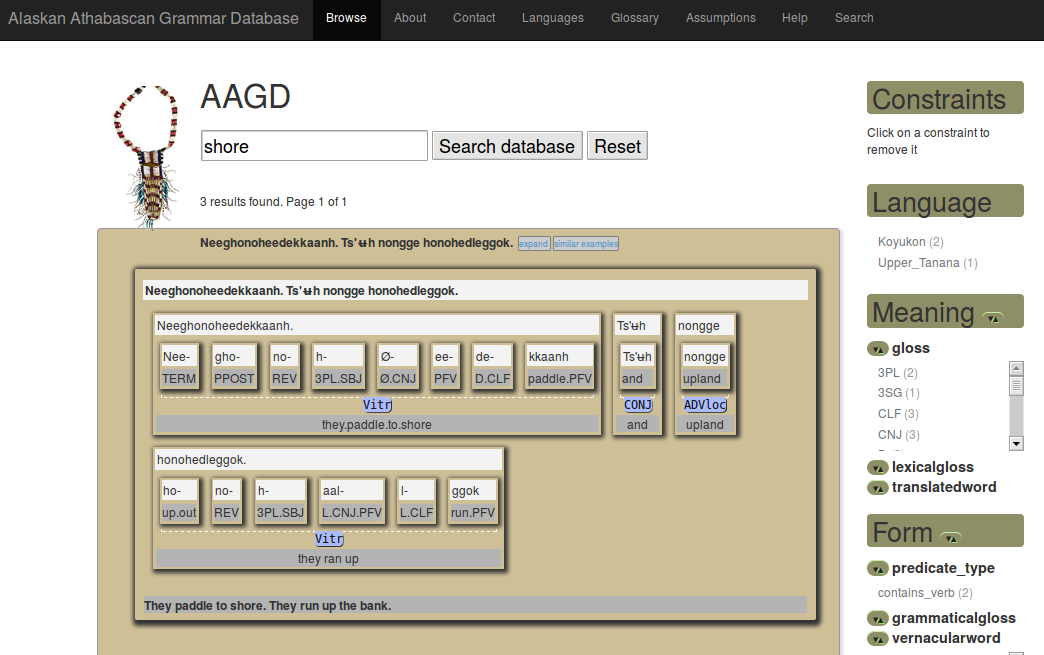
\includegraphics[width=\textwidth]{aagd.png}
\caption{Screenshot of the web frontend with a free text search, one fully visible example in the middle and faceted search on the right}
\end{figure}

\end{document}
